\subsection{Assortativity}
\label{subsec:assortativity}

As explained in section \ref{sec:matching}, the probability that two individuals are
matched can depend on background characteristics. In particular, we allow this
probability to depend on age and county of residence. While we do not have good data on
geographical assortativity and just roughly calibrate it such that 80\% of contacts are
within the same county, we can calibrate the assortative mixing by age from
\cite{Mossong2008}.

\begin{figure}[ht]
    \centering
    \begin{subfigure}[b]{0.425\textwidth}
        \centering
        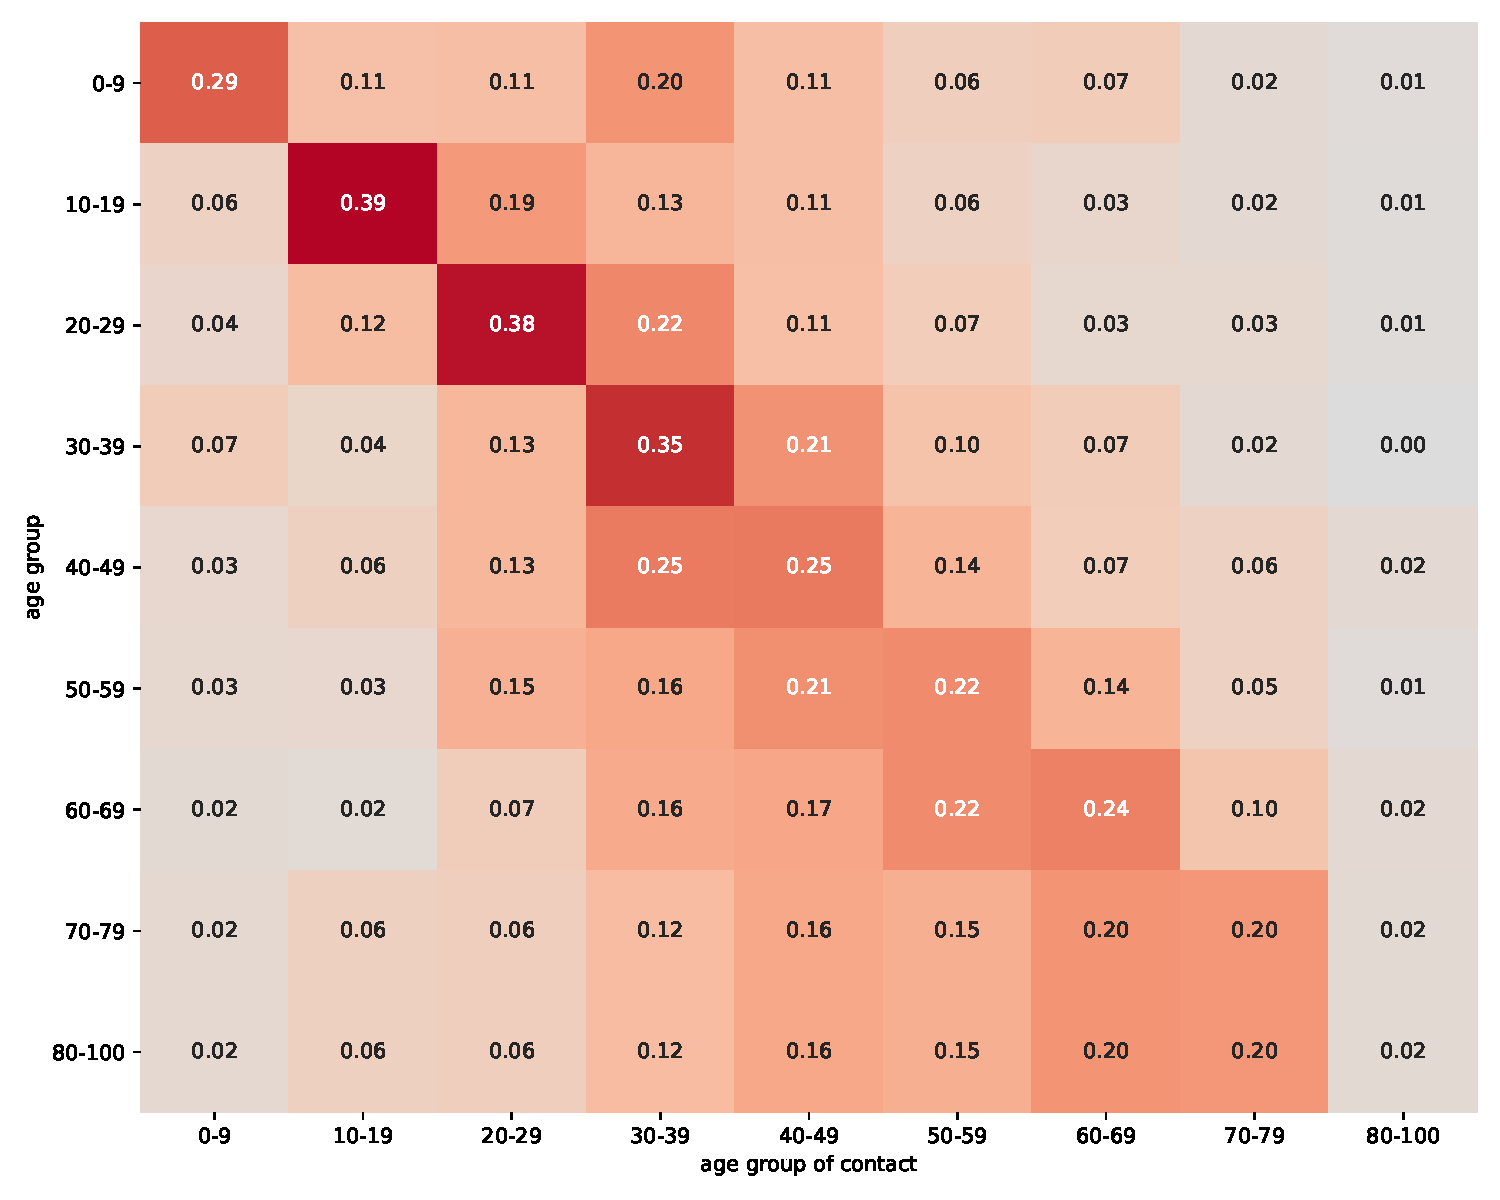
\includegraphics[width=\textwidth]{figures/results/figures/data/assortativity_other_non_recurrent}
        \caption{{Distribution of Non Recurrent Other Contacts by Age Group}}
        \label{fig:assortativity_other}
    \end{subfigure}
    \hfill
    % work assortativity
    \begin{subfigure}[b]{0.425\textwidth}
        \centering
        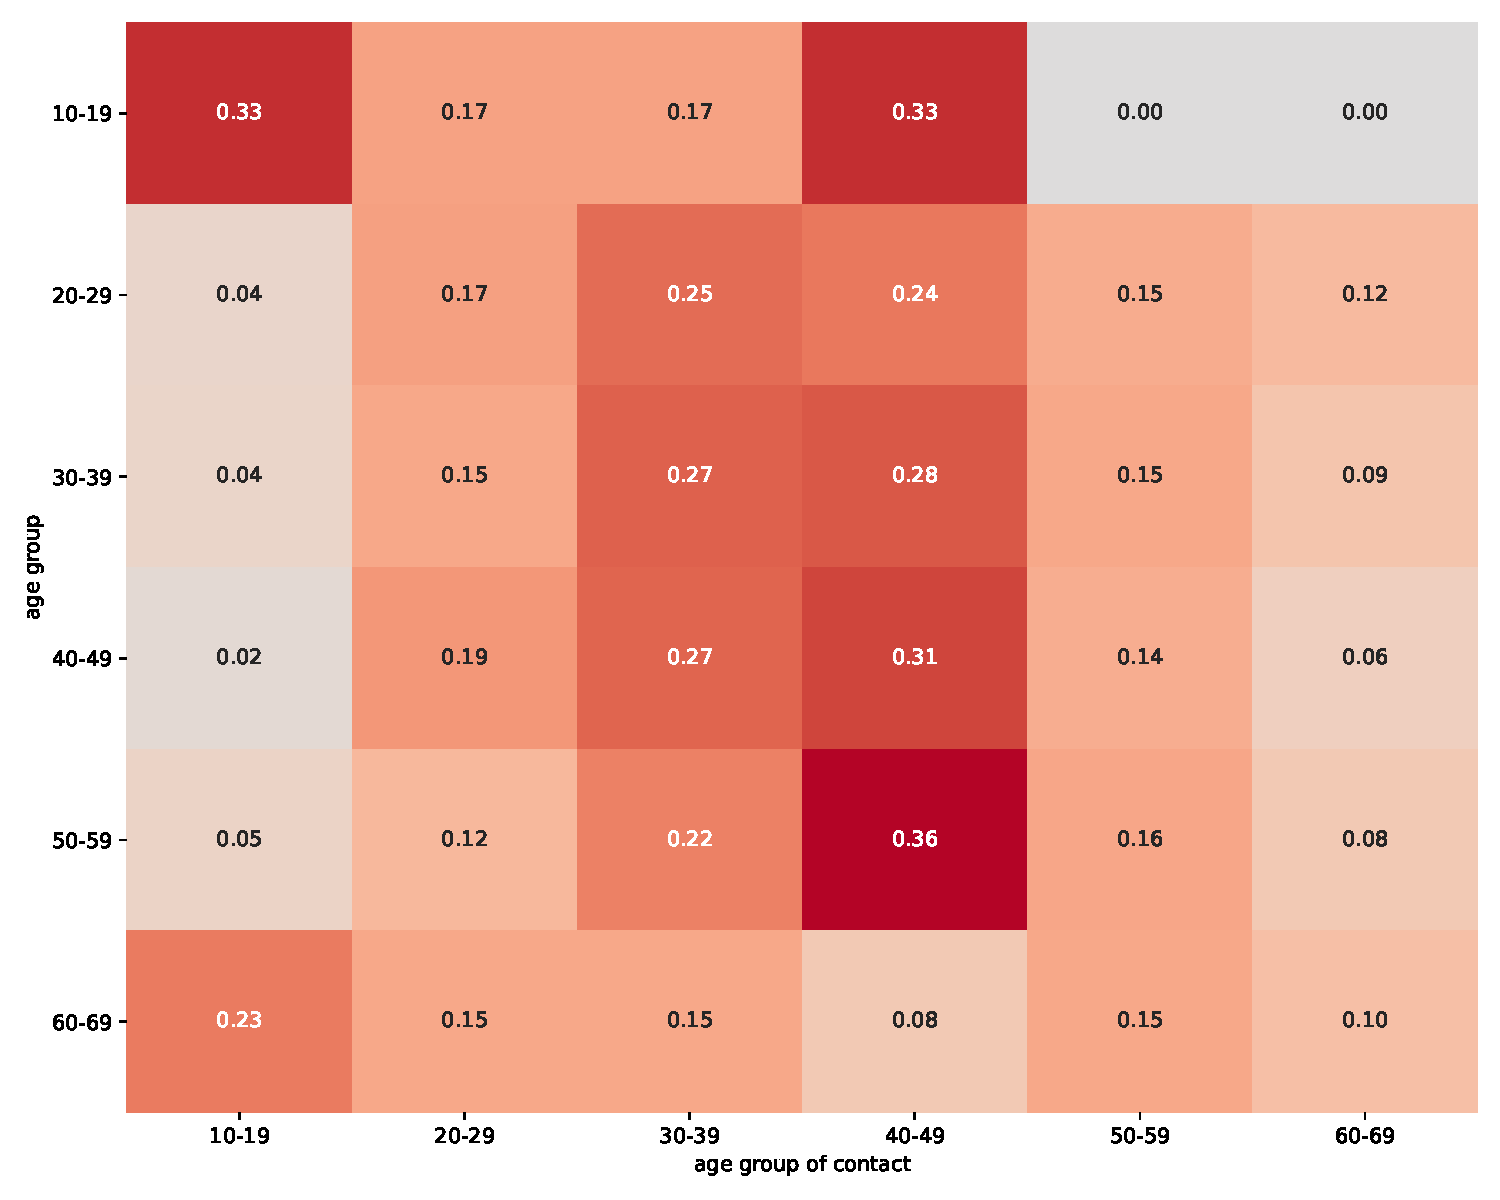
\includegraphics[width=0.9 \textwidth]{figures/results/figures/data/assortativity_work_non_recurrent}
        \caption{{Distribution of Non Recurrent Work Contacts by Age Group}}
        \label{fig:assortativity_work}
    \end{subfigure}

    \vskip3ex


    \caption{Assortativity by Age Group for Non Recurrent Other and Work Contacts}
    \floatfoot{\noindent \textit{Note:} The figure shows the distribution of non
        recurrent contacts by age group for other contacts on the left and work contacts
        on the right. A row shows the share of contacts a certain age group has with all
        other age groups. Higher values are colored in darker red tones. The diagonal
        represents the share of contacts with individuals from the same age group. The
        80-100 age group for other contacts was so small that we assumed for them to have
        the same contact distribution as the 70-79 year olds. For work contacts, we only
        show age groups that have a significant fraction of working individuals. The
        matrix must not be symmetric because the groups have very different sizes.}

    \label{fig:assortativity}

\end{figure}


Figure~\ref{fig:assortativity_other} shows that assortativity of the other contacts by
age is especially strong for children and adolescents. For older people, the pattern
becomes more dispersed around their own age group, but within-age-group contacts are
still the most common contacts. Figure~\ref{fig:assortativity_work} shows that
assortativity by age is also important among work contacts.

Our two other types of contacts, households and schools, get their assortativity by
construction. Schools are groups where the same children of the mostly same age and
county meet with teachers every day. Household composition follows directly from the
German microcensus data we use to construct our synthetic population.

\FloatBarrier